\documentclass{sig-alternate}

\usepackage[utf8]{inputenc}
\usepackage{enumitem}
\usepackage[hyphens]{url}
\usepackage[pdftex,urlcolor=black,colorlinks=true,linkcolor=black,citecolor=black]{hyperref}
\def\sectionautorefname{Section}
\def\subsectionautorefname{Subsection}

\usepackage{CJKutf8}

\newcommand{\superscript}[1]{\ensuremath{^{\textrm{#1}}}}

% listings and Verbatim environment
\usepackage[usenames,dvipsnames,svgnames,table]{xcolor}
\usepackage{fancyvrb}
\usepackage{relsize}
\usepackage{listings}
\usepackage{verbatim}
\newcommand{\defaultlistingsize}{\fontsize{8pt}{9.5pt}}
\newcommand{\inlinelistingsize}{\fontsize{8pt}{11pt}}
\newcommand{\smalllistingsize}{\fontsize{7.5pt}{9.5pt}}
\newcommand{\listingsize}{\defaultlistingsize}
\RecustomVerbatimCommand{\Verb}{Verb}{fontsize=\inlinelistingsize}
\RecustomVerbatimEnvironment{Verbatim}{Verbatim}{fontsize=\defaultlistingsize}
\lstset{frame=lines,captionpos=b,numberbychapter=false,escapechar=§,
        aboveskip=2em,belowskip=1em,abovecaptionskip=0.5em,belowcaptionskip=0.5em,
        framexbottommargin=-1em,basicstyle=\ttfamily\listingsize\selectfont}

% use Courier from this point onward
\let\oldttdefault\ttdefault
\renewcommand{\ttdefault}{pcr}
\let\oldurl\url
\renewcommand{\url}[1]{\inlinelistingsize\oldurl{#1}}

\lstdefinelanguage{JavaScript}{
  keywords={console, log, addEventListener, onmessage, alert, push, typeof, new, true, false, catch, function, return, null, catch, switch, var, if, in, while, do, else, case, break},
  keywordstyle=\bfseries,
  ndkeywords={class, export, boolean, throw, implements, import, this},
  ndkeywordstyle=\color{darkgray}\bfseries,
  identifierstyle=\color{Maroon},
  sensitive=false,
  comment=[l]{//},
  morecomment=[s]{/*}{*/},
  commentstyle=\color{ForestGreen},
  stringstyle=\color{Blue},
  morestring=[b]',
  morestring=[b]"
}

% linewrap symbol
\usepackage{color}
\definecolor{grey}{RGB}{130,130,130}
\newcommand{\linewrap}{\raisebox{-.6ex}{\textcolor{grey}{$\hookleftarrow$}}}

% todo macro
\usepackage{color}
\newcommand{\todo}[1]{\noindent\textcolor{red}{{\bf \{TODO}: #1{\bf \}}}}

\begin{document}
%
% --- Author Metadata here ---
\conferenceinfo{International World Wide Web Conference}{2014 Seoul, Korea}
\CopyrightYear{2014} % Allows default copyright year (20XX) to be over-ridden - IF NEED BE.
%\crdata{0-12345-67-8/90/01}  % Allows default copyright data (0-89791-88-6/97/05) to be over-ridden - IF NEED BE.
% --- End of Author Metadata ---

\title{Bots vs. Wikipedians, Anons vs. Logged-Ins:\\ A~Global Study of Edit Activity on Wikipedia and Wikidata}

\numberofauthors{1}

\author{
% 1st. author
\alignauthor
Thomas Steiner\titlenote{Thomas Steiner's second affiliation is \emph{Université de Lyon, CNRS Université Lyon~1, LIRIS, UMR5205, F-69622}}\\
       \affaddr{Google Germany GmbH}\\
       \affaddr{ABC-Str.~19}\\
       \affaddr{20354 Hamburg, Germany}\\
       \email{tomac@google.com}
}

\maketitle
\begin{abstract}
Wikipedia is a~global crowdsourced encyclopedia
that at time of writing is available in 287 languages.
Wikidata is a~likewise global crowdsourced knowledge base
that provides shared facts to be used by Wikipedias.
In the context of this research, we have developed
an application and an underlying
Application Programming Interface~(API) capable of monitoring
realtime edit activity of all language versions
of Wikipedia and Wikidata.
This application allows us to easily analyze edits
in order to answer questions such as
``Bots \emph{vs.}\ Wikipedians, who edits more?'',
``Which is the most anonymously edited Wikipedia?'',
or ``Who are the bots and what do they edit?''.
To the best of our knowledge,
this is the first time such an analysis
was done for Wikidata \emph{and}
for really \emph{all} Wikipedias---large and small.
According to our results, all Wikipedias \emph{and} Wikidata together
are edited by about 50\%~bots and by about 23\%~anonymous users.
Wikidata alone accounts for about 48\%~of the totally observed edits.
If we do \emph{not} consider Wikidata, \emph{i.e.},
if we \emph{only} look at all Wikipedias,
about 15\%~of all edits are made by bots
and 26\%~of all edits are made by anonymous users.
Overall, we found a~stabilizing number of 274~active bots
during our observation period.
Our application is available publicly online at the URL
\url{http://wikipedia-edits.herokuapp.com/},
its code has been open-sourced under the Apache~2.0 license.
\end{abstract}

\category{H.3.5}{Online Information Services}{Web-based services}

\terms{Human Factors, Languages, Measurement, Experimentation}

\keywords{Wikipedia, Wikidata, realtime monitoring, study, Web app}

\section{Introduction}

\paragraph{How Wikipedia Came to Life}

The fundamental shift from book-based encyclopedias
to CD-ROM-based encyclopedias
to finally Web-based encyclopedias
happened in the course of the 90ies
and started a~new era of freely and openly
available knowledge accessible to everybody.
The free online encyclopedia Wikipedia%
\footnote{Wikipedia: \url{http://www.wikipedia.org/}}~\cite{sanger05historywikipedia} was formally launched
on January 15, 2001 by Jimmy Wales
and Larry Sanger,
albeit the fundamental wiki technology and the underlying concepts are older.
Wikipedia's direct predecessor was Nupedia~\cite{sanger05historywikipedia},
a~similarly free online encyclopedia,
however, that was exclusively edited by experts
following a~strict peer-review process.
Wikipedia's initial role was to serve
as a~collaborative platform for draft articles for Nupedia.
What happened in practice was that Wikipedia rapidly overtook Nupedia
as there was no peer-review burden
and it is now a~globally successful Web encyclopedia
available in 287 languages with overall more than 30 million articles.%
\footnote{Wikipedia statistics: \url{http://stats.wikimedia.org/}}

\paragraph{International Expansion}

The international expansion began early on
in the project's existence,
with the first two non-English Wikipedias both
started on March 16, 2001 being the German and the Catalan ones,
followed briefly afterward by (Romanized) Japanese.
What followed was a~wave of new languages,
with French, Chinese, Dutch, Esperanto, Hebrew,
Italian, Portuguese, Russian, Spanish, Swedish,
Arabic, Hungarian, Afrikaans, Norwegian, and Serbian all being rolled out in the first year.

\paragraph{The First Wikipedia Bots}

Wikipedia bots are computer programs
with the purpose of automatically editing Wikipedia.
After occasional smaller-scale tests,
the first large-scale bot operation
was started in October 2002 by Derek Ramsey,%
\footnote{History of Wikipedia bots:
\url{http://bit.ly/History_Bots}}
who created a~bot to add a~large number
of articles about United States towns
based on tabular information
stemming from U.S. census data.
The generated articles used a~uniform
text template, so that all articles
followed the same writing style.
Today, bots are not only used to generate articles,
but also to fight vandalism and spam,
to correct typographic errors,
to improve references, and many more automatable tasks.%
\footnote{Wikipedia bots by purpose: \url{http://en.wikipedia.org/wiki/Category:Wikipedia_bots_by_purpose}}

\paragraph{The Knowledge Base Wikidata}

As Wikipedia is a~truly global effort,
sharing non-language-dependent facts
like population figures centrally
in a~knowledge base makes a~lot of sense
to facilitate international article expansion.
Wikidata\footnote{Wikidata: \url{http://www.wikidata.org/}}~\cite{vrandecic2012wikidata}
is a~free knowledge base that can be read
and edited by both humans and bots.
The knowledge base centralizes access to
and management of structured data,
such as references between Wikipedias
and statistical information that can be used in articles.
Controversial facts such as borders in conflict regions
can be added with multiple values and sources,
so that Wikipedia articles can,
dependent on their standpoint, choose preferred values.

\paragraph{Contributions}

The contributions of this paper are twofold.
On the engineering side, first, we have developed an application
and released its source code as open-source
that allows for realtime monitoring of all 287~Wikipedias and Wikidata.
Second, we have permanently made available a~publicly useable
Application Programming Interface~(API) that our application
is based upon and that we invite other interested parties to use.
On the research side, during the observation period
from November~4 to November~6, 2013,
we have monitored exactly
3,805,185~Wikipedia and Wikidata edits, 
out of which exactly 1,918,378~($\sim50.4\%$) were made by bots.
From the 3,805,185~total edits,
1,837,146~($\sim48.3\%$) can be allotted to Wikidata.
We have compiled global and local statistics on the impact of
bot edits \emph{vs.}\ human Wikipedian edits,
on anonymous human edits \emph{vs.}\ logged-in human edits,
and on bot activity in general.
In continuation, we have deep-dived into the data
and looked at the most \emph{bot-edited}, \emph{human-edited},
and \emph{anonymously-edited} Wikipedias and Wikidata.

\section{Methodology and Tools}

In our application, we make use of two enabling technologies,
namely the Wikipedia Recent Changes Internet Relay Chat~(IRC) feed
and a~push API called Server-Sent Events.

\paragraph{Wikipedia Recent Changes}
\label{sec:wikipedia-recent-changes}

Whenever a~human or bot changes an article
of any of the 287 Wikipedias,%
\footnote{List of Wikipedias by size:
\url{http://meta.wikimedia.org/wiki/List_of_Wikipedias}}
a~change event gets communicated by a~chat bot
over the Wikimedia IRC server (\url{irc.wikimedia.org}),%
\footnote{Raw IRC feeds of recent changes:
\url{http://meta.wikimedia.org/wiki/IRC/Channels\#Raw_feeds}}
so that parties interested in the data
can listen to the changes as they happen%
~\cite{steiner2013mjnomore}.
For each language version, there is
a~specific chat room following the pattern
\texttt{"\#" + language + ".wikipedia"}.
For example, changes to Catalan Wikipedia articles
will be streamed to the room \texttt{\#ca.wikipedia}.
An exception from this pattern is the room
\texttt{\#wikidata.wikipedia} for the language-independent
knowledge base Wikidata~\cite{vrandecic2012wikidata}.
A~sample original chat message with the components separated
by the asterisk character \texttt{`*'}
announcing a~change to an article
can be seen in the following.
\texttt{"[[Keep Calm and Carry On]] http://en.wikiped-\\ ia.org/w/index.php?diff=585806152\&oldid=585805943 \\* 74.197.171.148 * (+14) /* Parodies */"}.
The message components are \emph{(i)}~article name, \emph{(ii)}~revision URL,
\emph{(iii)}~Wiki\-pedia editor handle, and
\emph{(iv)}~change size and description.

\paragraph{Server-Sent Events}

Server-Sent Events~\cite{hickson2012sse}
defines an API for using an HTTP connection
to receive push notifications from a~server
in the form of DOM events.
Therefore, on the server side, a~script generates messages
of the MIME type \texttt{text/event-stream}
in an event stream format that can be seen
in \autoref{code:sse-server}.
The required event payload is in the \texttt{data:} field,
events can optionally be typed via a~proceeding \texttt{event:} field
and be uniquely identified via a~proceeding \texttt{id:} field.
The \texttt{data:} field allows no line breaks,
however, multiline messages are possible by prepending
a~separate \texttt{data:} string to each line.
Lines that start with a~colon are comments and are therefore ignored.
Consecutive events are separated by two line breaks.
The \texttt{EventSource} interface enables Web applications
to listen to pushed events from a~server over the HTTP protocol.
On the client side, using this API consists of creating
an \texttt{EventSource} object and registering event listeners,
as can be seen in \autoref{code:sse-client}.
When the client loses connection,
it automatically reconnects,
\emph{i.e.}\ without manual interaction.

\begin{figure}[h!]
\begin{lstlisting}[caption={Server-Sent Event of type ``enedit''
  (formatted for legibility, \texttt{data:} allows no line breaks)},
  label=code:sse-server, language=JavaScript]
: // Embedded JSON data without line breaks

id: 1386885965813
event: enedit
data: {
  "article": "Golden_Globe_Award_for_Best_§\linewrap§
      Actress_-_Motion_Picture_Musical_or_Comedy",
  "editor": "en:86.150.237.133",
  "isBot": false,
  "language": "en",
  "delta": "+9",
  "comment": "/* 2010s */",
  "diffUrl": "http://en.wikipedia.org/w/api.php?§\linewrap§
      action=compare&torev=585820379&fromrev=§\linewrap§
      585776128&format=json",
  "languageClusterUrl": "http://en.wikipedia§\linewrap§
      .org/w/api.php?action=query&prop=§\linewrap§
      langlinks&format=json&lllimit=500&§\linewrap§
      titles=Golden_Globe_Award_for_Best_§\linewrap§
      Actress_-_Motion_Picture_Musical_or_Comedy"
}
\end{lstlisting}

\begin{lstlisting}[caption={Creation of an \texttt{EventSource}
  object and registration of two event listeners},
  label=code:sse-client, language=JavaScript]
// connect to an SSE stream at relative URI /sse
var source = new EventSource('/sse');

// generic event listener for any Wikipedia edit
source.addEventListener('message', function(e) {
  var data = JSON.parse(e.data);
  console.log(e.lastEventId + ' ' + data.article);
}, false);

// listener for English Wikipedia edits
source.addEventListener('enedit', function(e) {
  var data = JSON.parse(e.data);
  console.log(e.lastEventId + ' ' + data.article);
}, false);
\end{lstlisting}
\end{figure}

\begin{figure}[h!]
  \centering
  \fbox{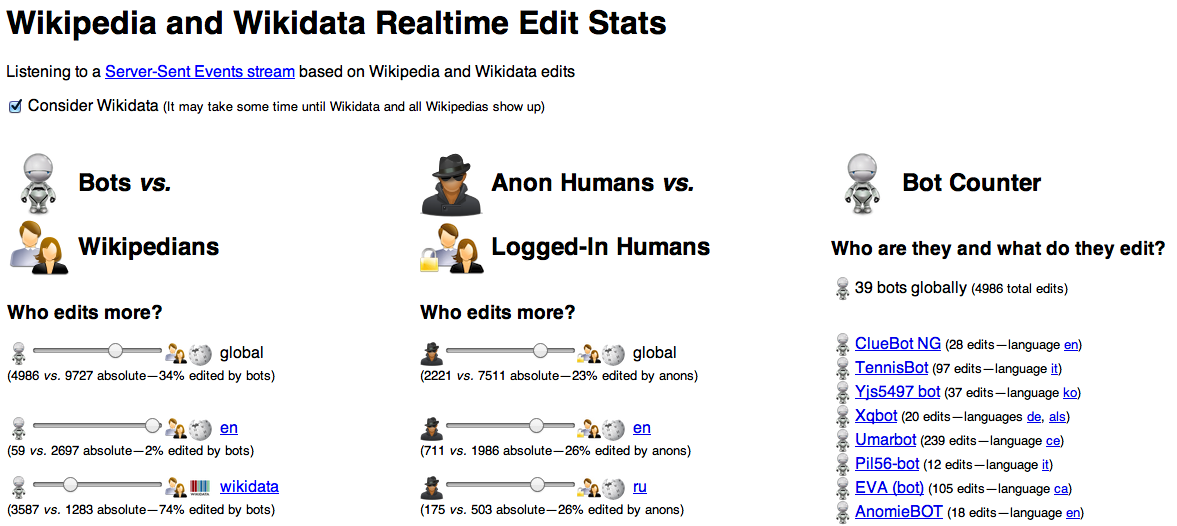
\includegraphics[width=\linewidth]{bots-vs-wikipedians.png}}
  \caption{Screenshot of the application available at \url{http://wikipedia-edits.herokuapp.com/} (cropped)}
  \label{fig:screenshot}
\end{figure}

\paragraph{Implementation Details}

Our application is based on a~Server-Sent Events API
that we have implemented in Node.js,
a~server side JavaScript software system
designed for writing scalable Internet applications.
%Programs are created using event-driven,
%asynchronous input/output operations
%to minimize overhead and maximize scalability.
Using Martyn Smith's Node.js IRC library,%
\footnote{Node IRC:
\url{https://github.com/martynsmith/node-irc}}
we listen for Wikipedia and Wikidata edit events
and send Server-Sent Events whenever we detect one.
Our API is available publicly online
at the URL \url{http://wikipedia-edits.herokuapp.com/sse}
and open for third parties to use.
On the client side,t in the actual application,
we have registered generic event handlers for events
pushed by the API and keep track of edit statistics over time.
This application can be tested at
\url{http://wikipedia-edits.herokuapp.com/}.\linebreak
A~screenshot of the application
can be seen in \autoref{fig:screenshot}.

\section{Results}

We have observed all 287~Wikipedias and Wikidata
during the observation period from November~4
to November~6, 2013.
While this may not sound like a~long time,
already during this short period
overall exactly 3,805,185~edit events occurred.
Our application updates in realtime,
which allows us to detect when relative figures,
\emph{i.e.}, percentages of bots \emph{vs.}\ Wikipedians
and anonymous \emph{vs.}\ logged-in humans start to converge.
This was the case after about half of the observation period.
At the end of the observation,
from all 287~Wikipedias and Wikidata,
exactly 260~($\sim90.3\%$) were edited,
which, given the long-long-tail of Wikipedias
with very few articles, justifies
our observation period duration.
Our application and underlying API being publicly available,
interested parties can run longer analyses at will.
In the following, we will zoom in on some interesting data points.
As a~side-remark---in consistence with
\autoref{sec:wikipedia-recent-changes}---%
we treat Wikidata like a~language when describing our results. 

\paragraph{Linearity of Number of Bots and Edits}

After the above-mentioned half of the observation period,
the number of bots \emph{vs.}\ the number of edits
started to grow in a~linear way, as can be seen in \autoref{fig:bots-total-edits}, which supports the fact that
relative figures from there on converged.

\paragraph{The Hockey Stick of Most Active Bots}

\autoref{fig:most-active-bots} shows a~classic hockey stick
curve of the most active bots.
Dexbot\footnote{Dexbot: \url{http://en.wikipedia.org/wiki/User:Dexbot}}
and ValterVBot\footnote{ValterVBot: \url{http://bit.ly/ValterVBot}} lead the field,
what follows next is a~long-tail of slowly declining bot activity
that, starting from KrBot, is roughly linear.
Dexbot and ValterVBot are both heavily active on Wikidata,
KrBot\footnote{KrBot: \url{https://ru.wikipedia.org/wiki/\%D0\%A3\%D1\%87\%D0\%B0\%D1\%81\%D1\%82\%D0\%BD\%D0\%B8\%D0\%BA:KrBot}}
is active on Wikidata and the Russian and Ukrainian Wikipedias.

\paragraph{The Few Linguistic Geniuses}

\autoref{fig:multilingual-bots} shows that only ten bots
are active in five languages or more, the clear leaders
being \begin{CJK}{UTF8}{min}タチコマ\end{CJK} robot%
\footnote{\begin{CJK}{UTF8}{min}タチコマ\end{CJK} robot:
\url{http://en.wikipedia.org/wiki/User:\%E3\%82\%BF\%E3\%83\%81\%E3\%82\%B3\%E3\%83\%9E_robot}} with 102~languages and
EmausBot\footnote{EmausBot:
\url{http://en.wikipedia.org/wiki/User:EmausBot}}
with 96~languages.
Both bots are consistently flagged as global bots.%
\footnote{Bots with global flag: \url{http://en.wikipedia.org/w/index.php?title=Special:GlobalUsers/Global_bot}}
A~large majority of 86\% of all bots are only active in one language.

\paragraph{The Linguae Francae of Wikipedia and Wikidata}

Given the previous results that only very few bots
act in more than one language, we asked ourselves
what were the languages that attracted the most bots.
\autoref{fig:bots-per-language} shows that the clear winners
are the English Wikipedia and Wikidata,
and, starting from the French Wikipedia, a~slow almost linear decline
in the number of active bots can be seen.
Overall only 5\% of all languages attracted more than ten bots.

\paragraph{The Relatively Most Bot-Edited Languages}

Requiring a~minimum threshold of 1,000 bot edits,
we looked at what were the relatively
(\emph{i.e.}, not absolutely) most bot-edited languages.
\autoref{fig:most-bot-edited-languages} shows the results,
with the fact that the Sindhi Wikipedia,
during the observation period, was 100\% bot-edited,
followed by the Sorani Wikipedia with 92\%
and Wikidata with 88\% bot activity.

\paragraph{The Relatively Most Human-Edited Languages}

Requiring a~minimum threshold of 1,000 human edits,
we looked at what were the relatively
most human-edited languages.
According to our results that can be seen in \autoref{fig:most-human-edited-languages},
during the observation period,
the Galician, the Slovenian, and the Javanese Wikipedias
were to 100\% human-edited, followed by
a~very smoothly descending stairway curve
with 31~languages being to 90\% or more human-edited.

\paragraph{The Relatively Most Anonymously-Edited Languages}

Looking at only human editors, we analyzed the relatively
most anonymously-edited languages, requiring a~minimum
number of 1,000 anonymous edits in order to be counted.
Our results depicted in \autoref{fig:most-anonymous-edited-languages}
show an almost linearly declining curve with the Thai,
the Korean, and the Simple English Wikipedias being at the top
with 41\% and twice 38\% anonymous editing activity
in the observation period. 

\paragraph{The Relatively Most Logged-In-Edited Languages}

\autoref{fig:most-logged-in-edited-languages} shows
the languages that had the most logged-in edits,
requiring a~minimum number of 1,000 logged-in edits.
The Javanese and the Esperanto Wikipedia together with Wikidata
mark the top logged-in-edited languages,
with the other languages declining approximately linearly.

\begin{figure}[p]
  \center
  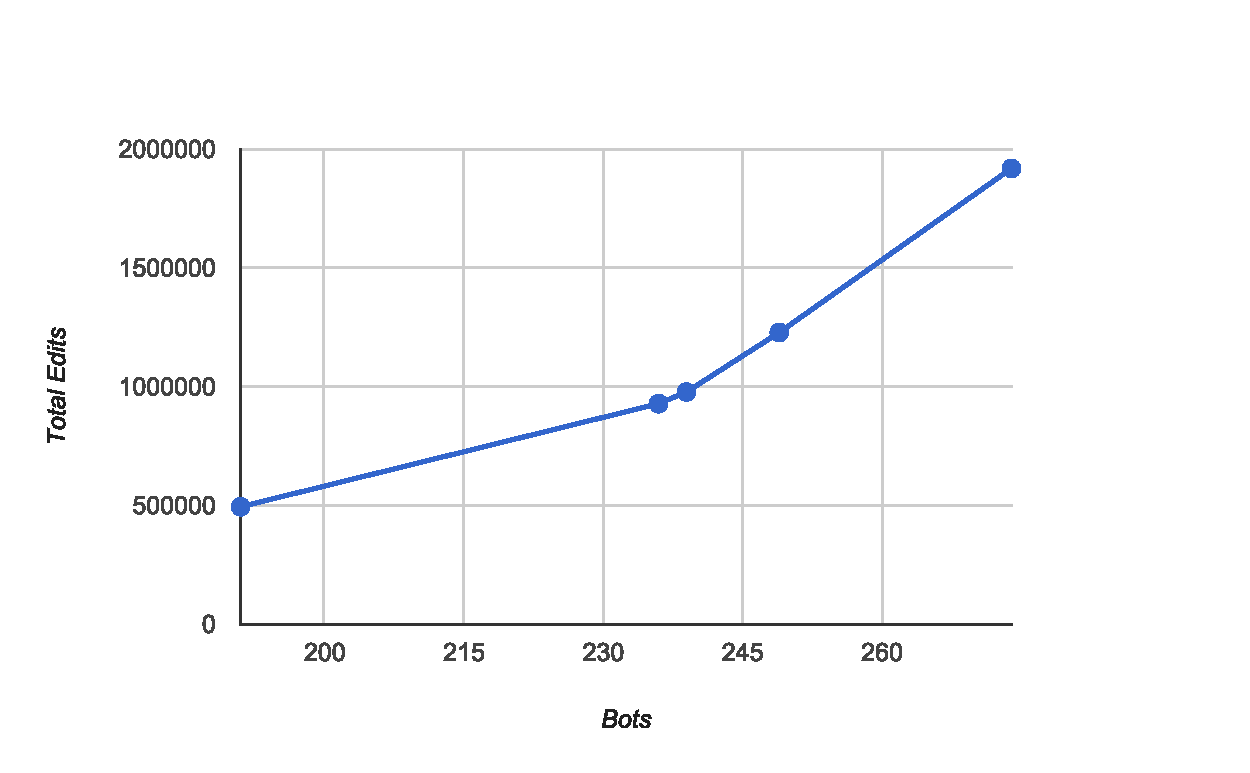
\includegraphics[width=0.84\linewidth]{bots-total-edits.pdf}
  \caption{Number of bots \emph{vs.}\ number of total edits}
  \label{fig:bots-total-edits}
\end{figure}

\begin{figure}[p]
  \center
  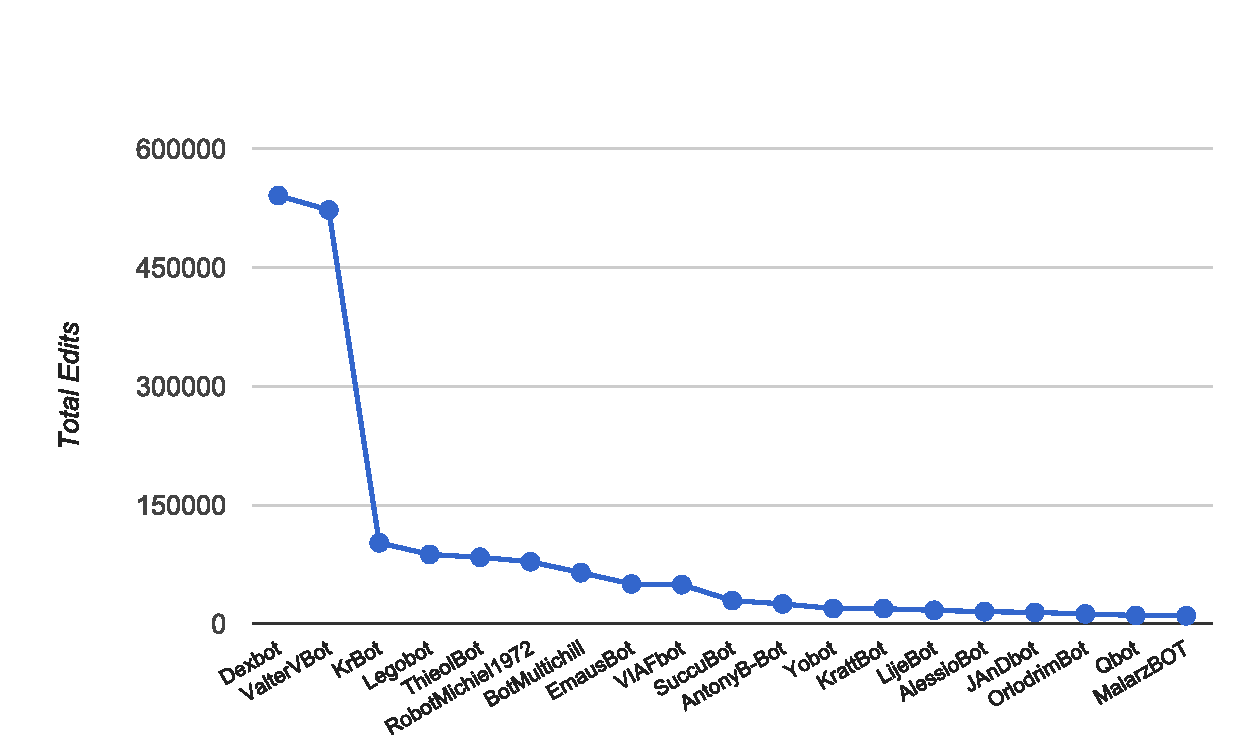
\includegraphics[width=\linewidth]{most-active-bots.pdf}
  \caption{Bots with more than 10,000 edits}
  \label{fig:most-active-bots}
\end{figure}

\begin{figure}[p]
  \center
  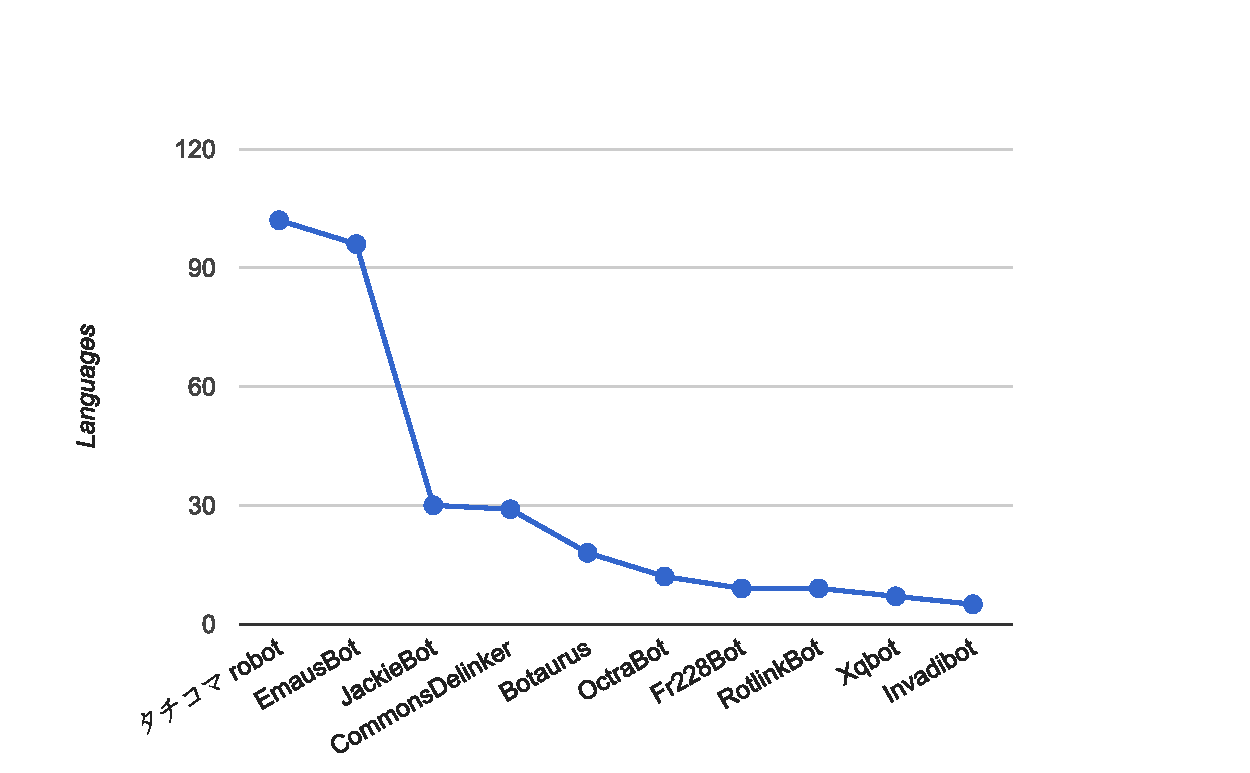
\includegraphics[width=\linewidth]{multilingual-bots.pdf}
  \caption{Multilingual bots active in $\geq5$ languages}
  \label{fig:multilingual-bots}
\end{figure}

\begin{figure}[p]
  \center
  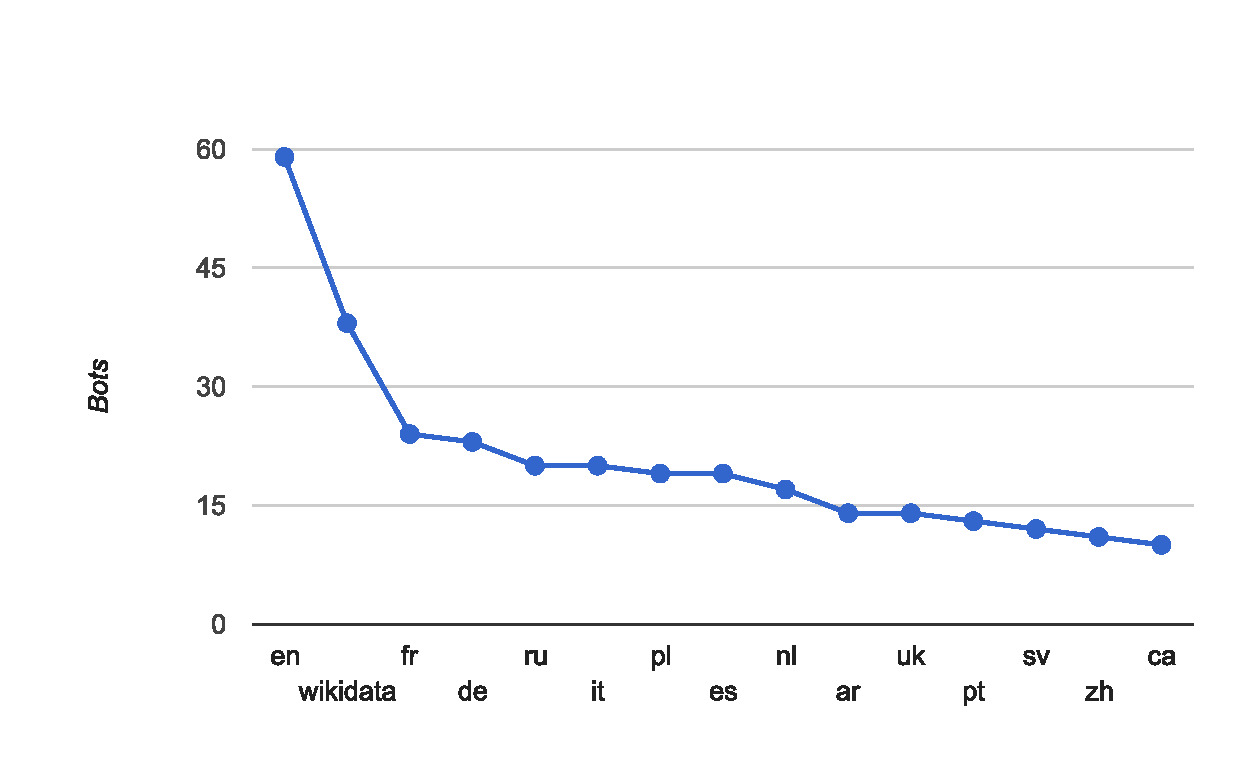
\includegraphics[width=0.9\linewidth]{bots-per-language.pdf}
  \caption{Languages with $\geq10$ active bots}
  \label{fig:bots-per-language}
\end{figure}

\begin{figure}[p]
  \center
  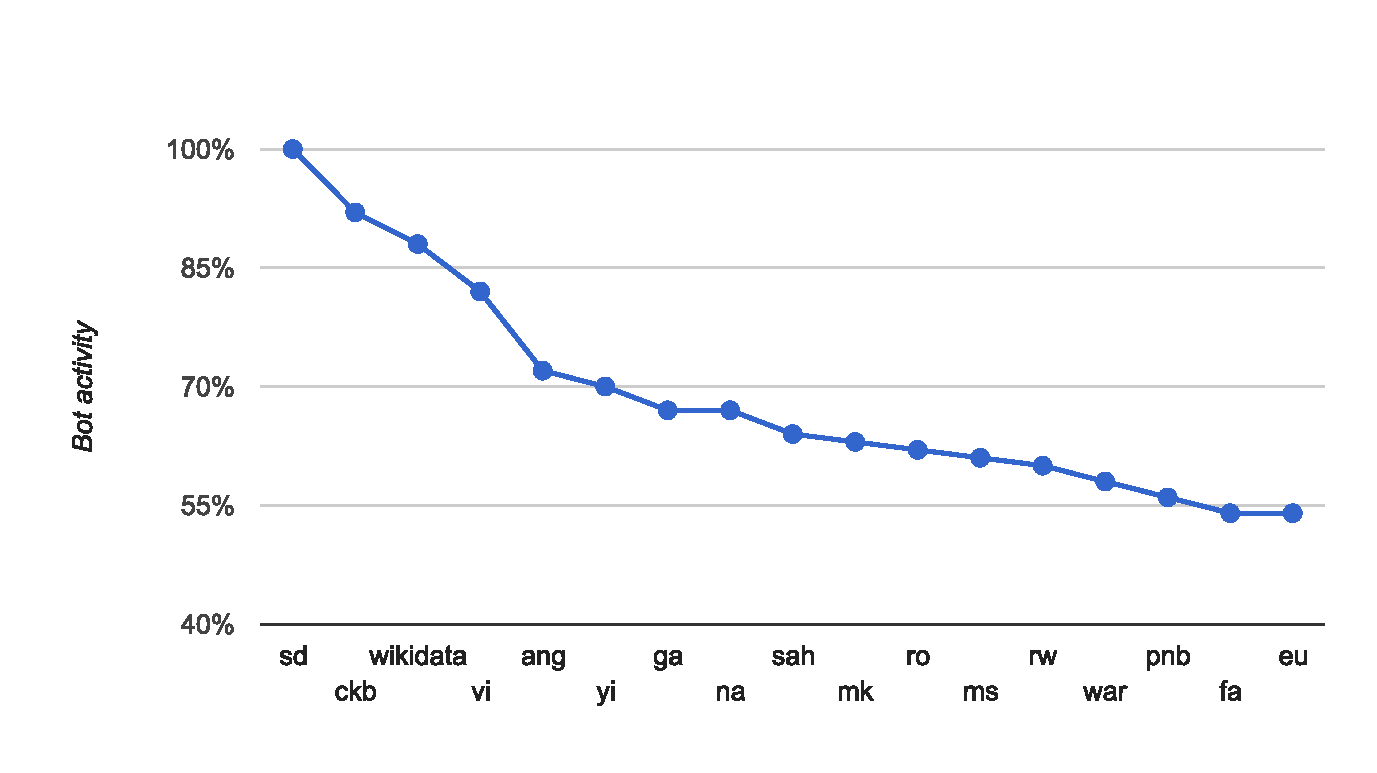
\includegraphics[width=0.9\linewidth]{most-bot-edited-languages.pdf}
  \caption{Percentage of bot activity $\geq50\%$ per language with $\geq1,000$ bot edits}
  \label{fig:most-bot-edited-languages}
\end{figure}

\begin{figure}[p]
  \center
  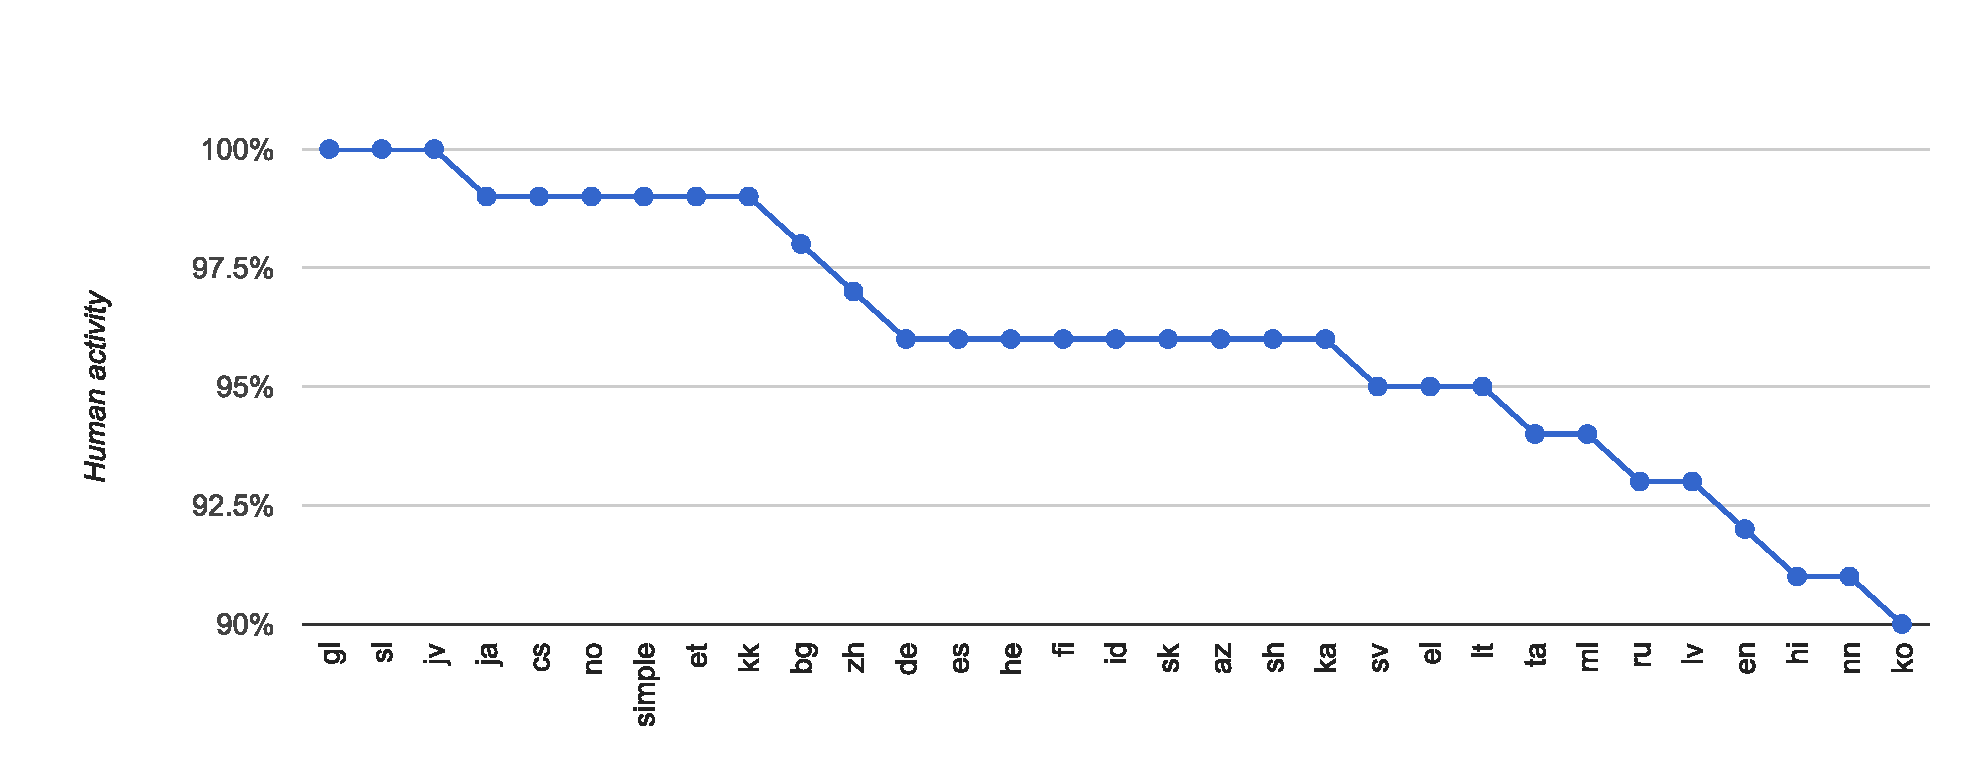
\includegraphics[width=\linewidth]{most-human-edited-languages.pdf}
  \caption{Percentage of human activity $\geq90\%$ per language with $\geq1,000$ human edits}
  \label{fig:most-human-edited-languages}
\end{figure}

\begin{figure}[p]
  \center
  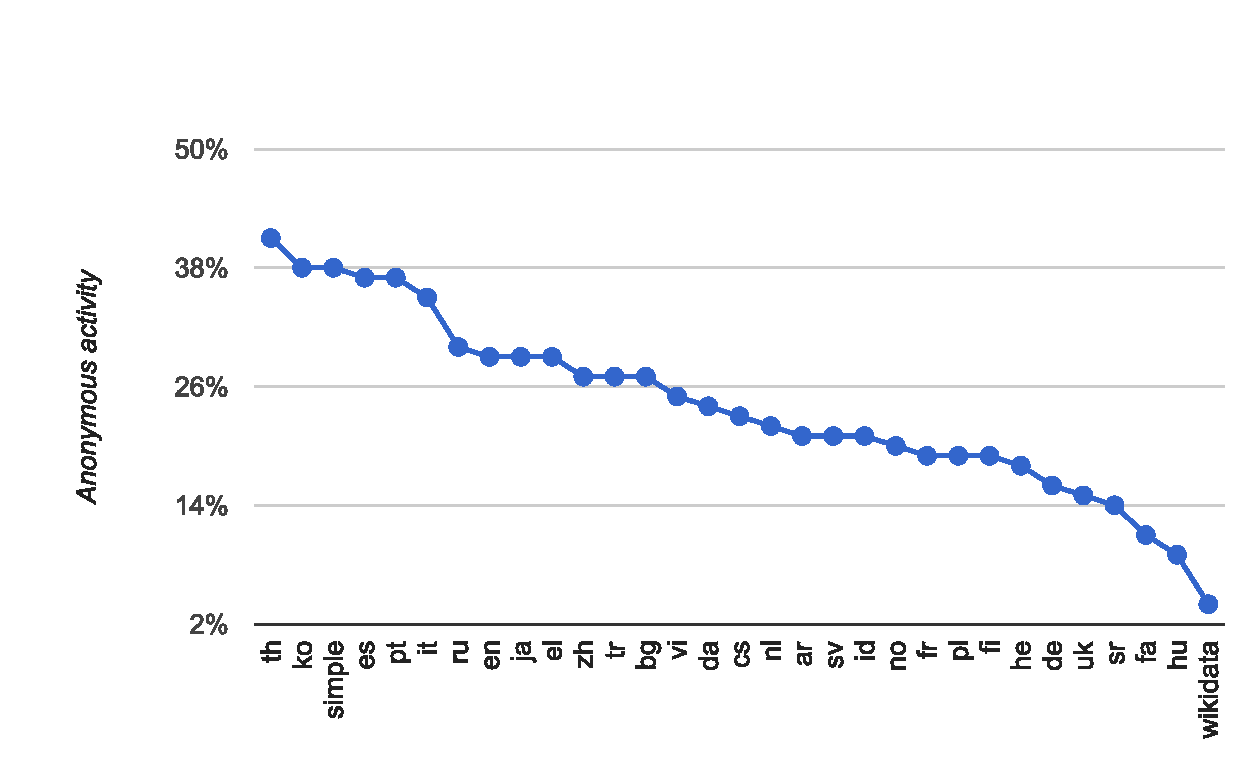
\includegraphics[width=\linewidth]{most-anonymous-edited-languages.pdf}
  \caption{Percentage of anonymous activity per language with $\geq1,000$ anonymous edits}
  \label{fig:most-anonymous-edited-languages}
\end{figure}

\begin{figure}[p]
  \center
  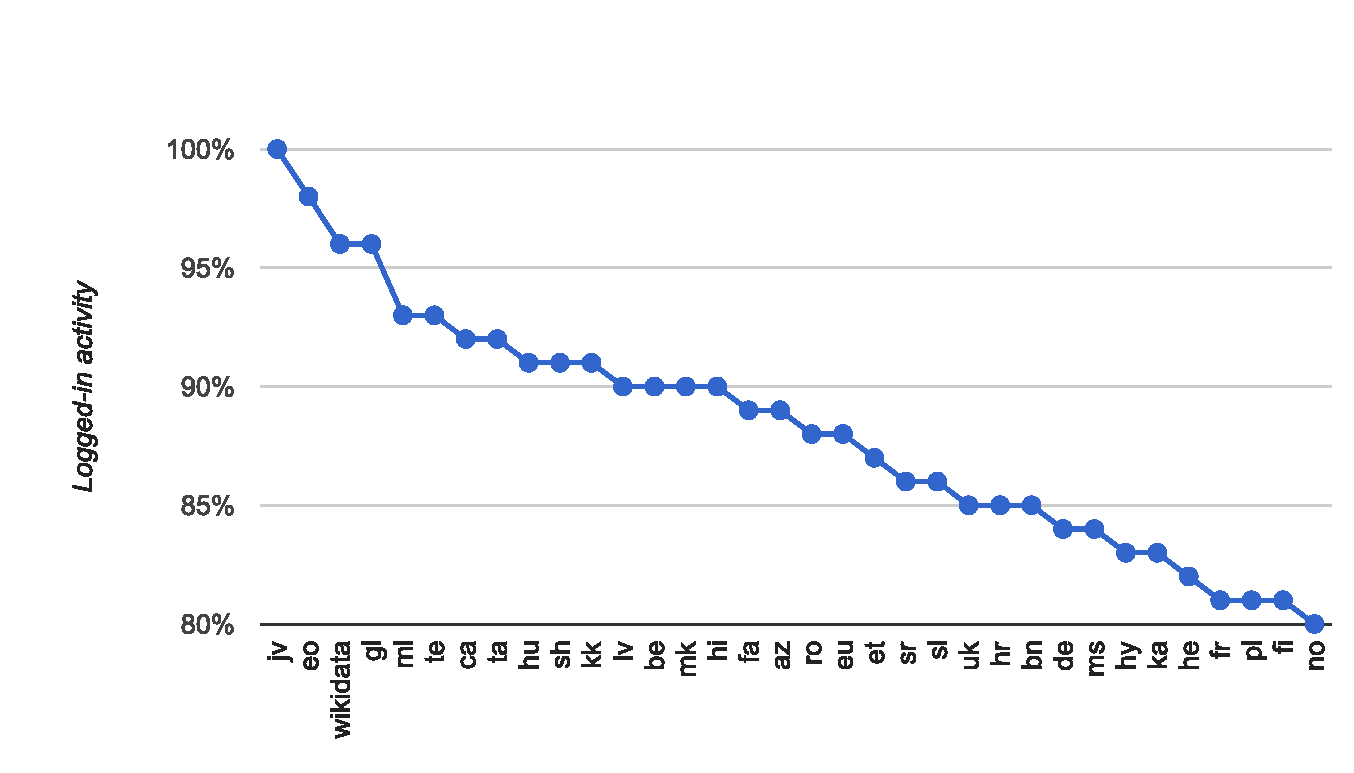
\includegraphics[width=\linewidth]{most-logged-in-edited-languages.pdf}
  \caption{Percentage of logged-in activity $\geq80\%$ per language with $\geq1,000$ logged-in edits}
  \label{fig:most-logged-in-edited-languages}
\end{figure}

\section{Discussion}

Interpreting and analyzing our obtained results,
there are some interesting discussion points.
We will deep-dive into some of them and provide interpretations
in the following.

\paragraph{The Long-Tail of Bots}

\autoref{fig:most-active-bots}, \autoref{fig:multilingual-bots},
and \autoref{fig:bots-per-language} all show a~tendency toward
hockey stick curves.
This implies that few outliers dominate
the long-tail rest.
Our results are in accordance with the work of Geiger \emph{et~al.}\
\cite{geiger2013withoutbots}, who have examined Wiki\-pedia 
quality control in the absence of the anti-vandalism bot ClueBot~NG%
\footnote{ClueBot~NG: \url{http://en.wikipedia.org/wiki/User:ClueBot_NG}}---%
according to our results
the 20\superscript{th}-most-active bot
and, at a~global view, still part of the hook
of the hockey stick.
Their results suggest that a~long-tail of bots
take over pending corrective tasks, however, at a~slower rate,
which acknowledges the importance of the long-tail.

\paragraph{Bots vs. Wikipedians}
\label{sec:bots-vs-wikipedians}

Bots on Wikipedia and Wikidata are used to make
repetitive automated edits
that would be extremely tedious to do manually.
It is interesting to compare the scales of the x- and y-axes of
\autoref{fig:most-bot-edited-languages} and
\autoref{fig:most-human-edited-languages}.
In the prior case (most bot-edited),
the y-scale goes from 40\% to 100\%
and the x-scale lists 17~languages.
In the latter case (most human-edited),
the y-scale goes from 90\% to 100\%
and the x-scale lists 33~languages.
What this implies is that the amount of languages dominantly edited by humans is a~lot higher than the amount
of languages dominantly edited by bots.
This suggests that while bots can reach quite
impressive qualities at contributing to Wikipedia~\cite{guldbrandsson2013bots},
overall humans still excel.

\paragraph{Anons vs. Logged-Ins}

It is a~well-known fact that the number of Wikipedia editors
has been declining in recent years%
~\cite{halfaker2013wikipedia}.
Looking at \autoref{fig:most-anonymous-edited-languages} and
\autoref{fig:most-logged-in-edited-languages},
we can observe a~similar trend as in the paragraph above.
The y-axis for the anonymously-edited languages
ranges from 2\% to 50\% with 31~languages listed on the x-axis,
compared to the y-axis for the most logged-in-edited languages
ranging from 80\% to 100\% with the x-axis listing 34~languages,
which implies that the amount of logged-in activity
greatly outperforms the amount of anonymous activity.
We leave comparing logged-in edits to anonymous edits 
open for future work, the hypothesis being that anonymous activity
is more likely to either be vandalism and spam%
~\cite{alfonseca2013spam} or smaller corrective edits,
whereas logged-in activity is more likely
going to produce quality content.

\section{Related Work}

The Wikimedia Foundation themselves provide
statistics for all Wikipedias
with ten or more articles and edits in the previous month%
~\cite{zachte2013wikipedia},
as well as statistics for Wikidata~\cite{zachte2013wikidata},
a~regular Wikipedia article on Wikipedia statistics%
~\cite{wikipedia2013stats},
and a~special auto-updating page on global high-level
Wikipedia statistics~\cite{wikipedia2013special}.
Statistics from~\cite{zachte2013wikidata} and~\cite{zachte2013wikipedia}
are based on recent database dump files
and contain a~note that \textit{``the lengthy dump process
(many weeks) means [that] a~delay in publishing these statistics
is always to be expected''}.
We accessed the statistics on December 13, 2013,
where the data was processed up until October 31, 2013.
Based upon the fact that these database dumps
of all Wikipedias are also publicly available,
in 2005 Voß~\cite{voss2005measuring} gave 
an overview on Wikipedia research
and analyzed articles, authors, edits, and links,
as well as content and quality.
A~similar study on Wikipedia research dating from 2006
has been conducted by Ayers~\cite{ayers2006researchingwikipedia}.
Unlike the methods described in~%
\cite{ayers2006researchingwikipedia,voss2005measuring,zachte2013wikidata,zachte2013wikipedia},
our approach works in realtime.
In~\cite{ciampaglia2010empiricalanalysis}, Ciampaglia and Vancheri
perform an empirical analysis of user participation
excluding bots in five large Wikipedias.
Adler \emph{et~al.}\ study in~\cite{adler2008measuringauthor}
various means to measure user contributions to Wikipedia.
As a~part of their study, they analyze bot editors
that, if they were included, created massive outliers
in the introduced measures.
In contrast to the approaches%
~\cite{adler2008measuringauthor,ciampaglia2010empiricalanalysis},
we do not exclude bots for our analysis,
but rather include them as equal citizens,
while at the same time still allowing for dynamically
disregarding them if need be.
Geiger and Halfaker study in~\cite{geiger2013withoutbots}
bot statistics and the effect
of the absence of a~popular anti-vandalism bot
on Wikipedia's quality control network.
The tool \emph{WikiChecker}\footnote{WikiChecker:
\url{http://en.wikichecker.com/}}
allows for near-realtime statistics
about logged-in \emph{vs.}\ anonymous users and more in
the English, French, Russian, and Japanese Wikipedias.
The application \emph{Wikipulse} shows realtime absolute
edit statistics for 36~Wikipedias, Wikimedia Commons, and Wikidata.
We provide detailed realtime statistics for all Wikipedias and Wikidata.
The \emph{Wikipedia Recent Changes Map} tool,
by LaPorte and Hashemi~\cite{laporte2013map},
inspired by a~similar too called \emph{WikipediaVision}%
~\cite{kozma2013map} by László Kozma,
takes the IP addresses of anonymous editors
of some of the biggest Wikipedias and maps them
in realtime to geolocations via a~lookup service.
We make the same information available
for all Wikipedias and Wikidata, however,
do not geolocate the IP addresses.
\emph{Listen to Wikipedia}~\cite{laporte2013listen}
is another project by
LaPorte and Hashemi that makes Wikipedia and Wikidata edits
audible and visualizes them in realtime.
Depending on the size, the kind of edit, or the editor status,
different sounds get played and colored circles displayed.
The application \emph{Wikistream}\footnote{Wikistream:
\url{http://wikistream.wmflabs.org/}} by Ed Summers
visualizes edits on all Wikipedias and Wikidata
in realtime and uses recently uploaded images from Wikimedia Commons
as background images, but does not keep track of edit statistics.
Several tools provide processed page view statistics
based on database dumps, examples are
\emph{Wikipedia article traffic statistics}%
\footnote{Wikipedia article traffic statistics:
\url{http://stats.grok.se/}} by ``User:Henrik'',
\emph{Wikipedia article traffic statistics}%
\footnote{Wikipedia article traffic statistics:
\url{http://toolserver.org/~emw/wikistats/}} by ``User:Emw'',
or finally \emph{Wikipedia Page Views}%
\footnote{Wikipedia Page Views: \url{http://wikistats.ins.cwi.nl/}}
by Hannes Mühleisen.
Mestyán \emph{et~al.}~\cite{mestyan2013boxoffice} measure and analyze the activity level of editors and viewers in order
to predict the box office success of movies.
We do not focus on page view statistics based on database dumps,
but realtime article edit statistics instead.
In~\cite{boukhelifa2010realtime}, Boukhelifa \emph{et~al.}\
classify statistics tools in the categories global and local.
According to this classification,
local tools focus on individual articles or users
and therefore require time-consuming on-the-fly computations.
In contrast,  global tools
show the evolution of aggregated data
for all Wikipedias,
but without acquiring realtime data.
According to this classification, our approach can be
classified as global, however, with realtime support.

\section{Conclusions and Future Work}

We have introduced an application
and underlying API for the realtime monitoring
of all 287~Wikipedias and Wikidata.
Via this application, which was also open-sourced under the Apache~2.0 license,
we have collected more than 3.8~million edit events
that we have analyzed in order to get a~better understanding
of Wikipedia and Wikidata editors.
This allowed us to get a~feeling of the relations of
logged-in \emph{vs.}\ anonymous edits
and edits made by bots \emph{vs.}\ edits made by humans
globally and locally.
We have looked at bots and their languages
and created several analyses based thereon.

Future wok has several possible directions.
On the engineering side, we want to improve the application
such that it creates the diagrams shown in this paper directly.
Further, we envision a~global bot health check system
that, based on the regular bot behavior patters,
tries to detect outliers caused by
potentially rogue bots or failing bots,
so that we can alert adminstrators early on
\textit{``when the levee breaks''}~\cite{geiger2013withoutbots}.
On the research side, an interesting step to take
is to look at qualitative differences
between bot edits and human edits, and for the latter,
logged-in and anonymous edits.
While we now have a~feeling about relative and absolute numbers,
looking into the contents of the actual edits---%
which our API allows, as for each edit event it sends the
\texttt{diffUrl} and \texttt{languageClusterUrl}
(see \autoref{code:sse-server})---%
opens many research opportunities ranging from spam
and vandalism detection~\cite{alfonseca2013spam}
to realtime article tracking for monitoring events
as they happen on Wikipedia~\cite{steiner2013mjnomore}
or even disaster response.
Like with Twitter's Streaming APIs%
\footnote{Twitter Streaming APIs:
\url{https://dev.twitter.com/docs/streaming-apis}}
that people have found creative uses for%
~\cite{petrovic2010streamingfirststory},
our API can facilitate interesting use cases
for data from Wikipedia and Wikidata like the detection of
edit wars~\cite{yasseri2012conflicts}
reflecting real-world conflicts.

Concluding, we have contributed a~useful
Wikipedia and Wikidata monitoring tool
as well as an open API
and have performed an initial global study 
with interesting and surprising insights that
expectedly will be the first in a~series
of many more future studies and applications by us
and others.
 
\bibliographystyle{abbrv}
\bibliography{references}
\balancecolumns
\end{document}
